\documentclass[11pt, a4paper]{article}
\usepackage[utf8]{inputenc}
\usepackage[margin=1in]{geometry} %Sets proper 1-inch margins. 
\usepackage{amsmath} %Only load this if you are using math/equations.
\usepackage{graphicx} %Only need to call this if inserting images.
\usepackage{caption} %Only need to call this if inserting captions.
\usepackage{float} %Allows the use of the [H] specifier. 
%\graphicspath{{C:/Users/jonah/Pictures/}} %Sets the working directory for images.
\usepackage[colorlinks,citecolor=blue,linkcolor=blue,urlcolor=blue]{hyperref} %Allows for the embedding of urls. 
\usepackage{setspace}
\usepackage{blindtext}

\pagenumbering{arabic}

%\usepackage{fontspec} %%in order for this font stuff to work, you must compile using xelatex+makeindex+bibtex (or at minimum xelatex)
%\setmainfont[Mapping=tex-text-ms]{Essays1743}

\usepackage{fancyhdr}

\pagestyle{fancy}
\fancyhf{}
\rhead{Greenough \& Edmundson \\ 2023}
\lhead{\thepage}

\newcommand{\comment}[1]{}

\usepackage{Sweave}
\begin{document}
\Sconcordance{concordance:project_report.tex:project_report.Rnw:%
1 26 1 1 0 26 1 1 23 12 1 1 3 3 0 1 1 7 0 1 1 3 0 1 7 2 1 1 5 3 0 1 1 6 %
0 1 1 3 0 1 2 2 1 1 11 1 4 13 0 1 2 8 1 1 8 30 0 1 2 1 5 7 1 1 9 2 1 1 %
3 19 0 1 2 4 1 1 7 4 0 1 5 4 0 1 2 12 1 1 5 3 0 1 1 3 0 1 1 1 0 1 2 2 1 %
2 2 2 1 2 2 7 1 1 5 2 2 2 1 2 2 2 1 1 2 3 0 1 6 1 0 1 2 6 1 1 3 3 0 1 3 %
1 0 1 2 4 1 1 2 3 0 1 3 1 0 1 2 5 1 1 7 2 1 1 2 3 0 2 3 1 4 1 2 1 1 1 %
19 2 1 1 18 3 0 1 1 9 0 1 1 3 0 1 2 16 1}


\begin{center}
\LARGE{DATA583 Project Report}
\par
\vspace{1.0pc}
\par
\large{Madison Greenough \& Jonah Edmundson}
\end{center}


\vspace{0.917 pc} %Creates a paragraph line break. 

%\pagebreak

%\tableofcontents

%\pagebreak
\section{Dataset Introduction and Hypotheses}

This dataset was scraped from \href{https://www.trulia.com/NY/New\_York/20\_p/}{Trulia}, and it contains 800 recently posted real estate listings in New York City. The variables contain information on the listing, including the \texttt{price} (integer in \$USD), \texttt{bedrooms} (numeric, int), \texttt{bathrooms} (numeric), \texttt{feet} (numeric), \texttt{address} (string), \texttt{newflag} (binary 0 or 1), \texttt{listing company} (string), \texttt{latitude} (numeric), \texttt{longitude} (numeric), and \texttt{distance} to Central Park (numeric). The distance metrics were computed by mapping the address and converting to coordinates and then calculating the distance to a central location, Central Park.

The purpose of this report is to attempt to model price as a response variable given the dependent variables in the dataset mentioned above. Determining a well-fitting model will allow for the model to be used to make predictions for future listing prices. This would serve many purposes, as it would act as a tool for listing companies when appraising a home to determine the list price. It could also be used by buyers to determine their offer price for a property given its features, and it could help to identify if the listing is priced appropriately or not.

We hypothesize that clustering will prove to be a suitable model to help predict prices given the input variables, and we also expect that it will help map these listing onto a map of the city, to be used by the clustering algorithm when grouping by boroughs. Note that there are five main boroughs in New York City, consisting of Staten Island, Brooklyn, Queens, Manhattan, and the Bronx. Naturally, we would expect that some of these neighbourhoods will fetch higher prices for properties, as it is common knowledge that Manhattan, for example, is an exclusive neighbourhood. We also expect that larger quantities of bedrooms and bathrooms will fetch higher list prices. Additionally, a larger square footage, or size, of the listing will also increase the price. We expect that as the distance to Central Park increases, the price will decrease, as we predict that this is a desired location. Throughout this report, we will be fitting various statistical models to attempt to represent the relationship between price and the other variables, and to determine whether or not our hypotheses are correct.


\pagebreak

\section{Analysis}

A comprehensive analysis was conducted by fitting several different statistical models to test the fit. Many different models and tools were fitted but not shown due to the lack of application and relevance to our hypotheses. Below, see a few of the models fitted that were beneficial to our analysis.

\subsection{Modelling Price}

\subsubsection{Multiple Linear Regression}

First, a multiple linear regression model (MLR) was fitted with all coefficients. Note that our response variable, \texttt{price}, was used in the model as a log value. Below see a quick summary output of just the coefficient statistics as well as the $R^2$. Note that the p-values were very small for \texttt{bath} and \texttt{distance}, but not for \texttt{bed} and \texttt{feet}. The $R^2$ value of 0.554 was poor, indicating that nearly half of the variability in the data is not captured by this model.

\begin{Schunk}
\begin{Soutput}
Full model coefficients:
\end{Soutput}
\begin{Soutput}
                 Estimate   Std. Error      t value     Pr(>|t|)
(Intercept)  5.825061e+00 2.661874e-02 218.83308451 0.000000e+00
bed          2.500316e-04 9.620429e-03   0.02598965 9.792782e-01
bath         1.569572e-01 1.384433e-02  11.33729711 4.217251e-26
feet         2.188341e-05 9.347670e-06   2.34105564 1.970765e-02
distance    -1.724545e-02 1.335443e-03 -12.91365594 3.009396e-32
\end{Soutput}
\begin{Soutput}
Full model R^2: 0.554
\end{Soutput}
\end{Schunk}

The next linear model fitted was a best subset. This model was created by using the BIC values to determine the best subset of the variables used in the first multiple linear regression model above. Looking below, we see that there are just two coefficients remaining, \texttt{bath} and \texttt{distance}. Note that these are the same two coefficients that were the most significant in the first model. Both coefficients are very significant, but the $R^2$ is still very poor, at just 0.55.

\begin{Schunk}
\begin{Soutput}
Best subset coefficients:
\end{Soutput}
\begin{Soutput}
$coefficients
               Estimate  Std. Error   t value     Pr(>|t|)
(Intercept)  5.82872668 0.026596100 219.15719 0.000000e+00
bath         0.17116399 0.008497619  20.14258 2.613608e-63
distance    -0.01714561 0.001300845 -13.18036 2.399164e-33
\end{Soutput}
\begin{Soutput}
Best subset R^2: 0.55
\end{Soutput}
\end{Schunk}

Using the consistent model specification test, we tested the linear models to the null model. Below, the results outline that the p-value is significant so the null of correct specification is rejected at the 0.1\% level.


\begin{Schunk}
\begin{Soutput}
Consistent Model Specification Test
Parametric null model: lm(formula = logprice ~ bed + bath + feet + distance,
                          data = no_outliers, x = TRUE, y = TRUE)
Number of regressors: 4
IID Bootstrap (399 replications)

Test Statistic ‘Jn’: 12.01751	P Value: < 2.22e-16 ***
---
Signif. codes:  0 '***' 0.001 '**' 0.01 '*' 0.05 '.' 0.1 ' ' 1
Null of correct specification is rejected at the 0.1% level
\end{Soutput}
\end{Schunk}

Given the poor results from the linear models, it can be concluded that this approach will not best represent our data. Moving forward, we will look at a GLM model.

\subsubsection{General Linear Model}

First, a general linear model (GLM) model was fitted with all coefficients. Note that our response variable, price, was used in the model as a log value. Below see a summary output of this model fitted with Gaussian distribution. Notice that \texttt{bed} is very insignificant, but the other three variables are significant. The \texttt{residual deviance} value is significantly smaller than the degrees of freedom, which indicates it may not be the best model fit. 

Additionally, we see a plot that maps the density of the original price data compared to the density of normal distribution with the dataset's mean and standard deviation. We see that the fit is not the best, as the lines do not follow the same relative distribution.

\begin{Schunk}
\begin{Soutput}
Call:
glm(formula = logprice ~ bed + bath + feet + distance, family = gaussian(link = "identity"), 
    data = no_outliers, x = TRUE, y = TRUE)

Deviance Residuals: 
     Min        1Q    Median        3Q       Max  
-0.99160  -0.15656   0.01398   0.15362   0.64337  

Coefficients:
              Estimate Std. Error t value Pr(>|t|)    
(Intercept)  5.825e+00  2.662e-02 218.833   <2e-16 ***
bed          2.500e-04  9.620e-03   0.026   0.9793    
bath         1.570e-01  1.384e-02  11.337   <2e-16 ***
feet         2.188e-05  9.348e-06   2.341   0.0197 *  
distance    -1.725e-02  1.335e-03 -12.914   <2e-16 ***
---
Signif. codes:  0 ‘***’ 0.001 ‘**’ 0.01 ‘*’ 0.05 ‘.’ 0.1 ‘ ’ 1

(Dispersion parameter for gaussian family taken to be 0.05466844)

    Null deviance: 50.773  on 414  degrees of freedom
Residual deviance: 22.414  on 410  degrees of freedom
  (372 observations deleted due to missingness)
AIC: -21.496

Number of Fisher Scoring iterations: 2
\end{Soutput}
\end{Schunk}
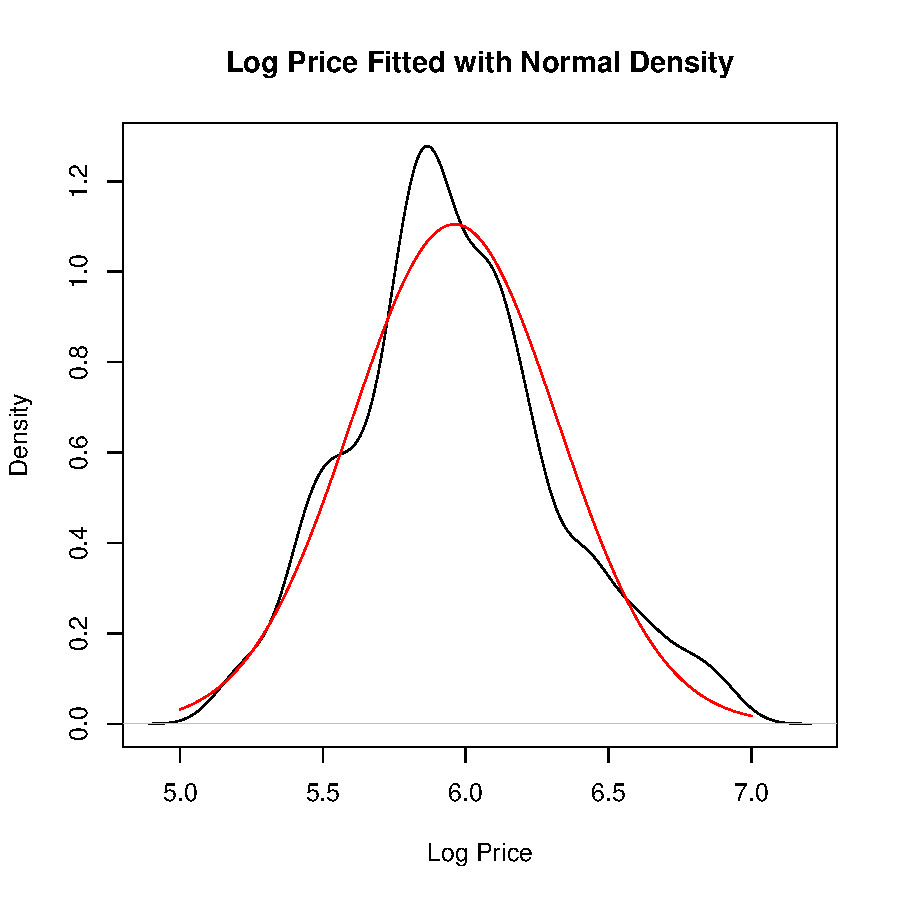
\includegraphics{project_report-006}


Given this output and due to the fact that the deviance is quite far off of the degrees of freedom, it is safe to say that this glm fit is not the best model for the dataset. A non-parametric approach is the next step in our model fitting process. 


\subsubsection{Nonparametric Approach}

Our next attempt at modelling price was through a non-parametric regression approach. Here, we conducted a Kernel Regression Significance Test which tested our variables \texttt{distance, feet, bed, bath}. The output for this data is shown below. First, the bandwidths are given which indicates that the \texttt{feet} bandwidth is very large compared to the other three. \texttt{Bath} is the smallest by far, with just 0.15. The individual significance test show the p-value which indicates that \texttt{bed} is very significant, \texttt{bath} is moderately significant, but \texttt{distance} and \texttt{feet} are not. Overall, this model fit appears to be the best approach so far.




\begin{Schunk}
\begin{Soutput}
Kernel Regression Significance Test
Type I Test with IID Bootstrap (399 replications, Pivot = TRUE, joint = FALSE)
Explanatory variables tested for significance:
distance (1), feet (2), bed (3), bath (4)

              distance     feet       bed      bath
Bandwidth(s): 1.791452 157.5778 0.9999986 0.1562374

Individual Significance Tests
P Value: 
distance 0.278195  
feet     0.776942  
bed      0.010025 * 
bath     < 2e-16 ***
---
Signif. codes:  0 '***' 0.001 '**' 0.01 '*' 0.05 '.' 0.1 ' ' 1
\end{Soutput}
\end{Schunk}

Now that all of the attempts to model price have been completed and we can compare them amongst each other.

Below, we see the mean squared estimates (MSE) and $R^2$ values for the models calculated so far. We see that the man squared estimates are all very large, with the MLR and GLMs the largest and quite similar, with the Kernel MSE smaller but still very large. The $R^2$ values for the MLR and GLM, recall, are quite poor, with just over half of the variation explained by the model. The Kernel $R^2$ value is significantly better, with 0.94 approximately. This indicates that the Kernel model has been the best for modelling price. 

\begin{Schunk}
\begin{Soutput}
       MLR.MSE      GLM.MSE   Kernel.MSE
1 4.236895e+12 4.236895e+12 131586687935
\end{Soutput}
\begin{Soutput}
     MLR.R2    GLM.R2 Kernel.R2
1 0.5585456 0.5585456 0.9393155
\end{Soutput}
\end{Schunk}



\pagebreak
\subsection{Clustering}
%https://data.cityofnewyork.us/City-Government/Borough-Boundaries/tqmj-j8zm

This next portion will walk through the different clustering methods attempted to fit the dataset with respect to the distance metrics.

\subsubsection{Hierarchical}

First, hierarchical clustering was conducted on the dataset. Recall the 5 main boroughs in New York City that was mentioned earlier. This data was segmented into 5 clusters with this model. Below see the the table output for the count of listings allocated to each of the 5 clusters. Additionally, see below the dendogram for the hierarchical cluster fitted with a complete method used. The dendogram visualizes the distance of the points when they were clustered. It can be seen here, around the height of 0.5, that the clusters are in 5 main groups, or clusters. Note that in this model, the clustering was run on \texttt{latitude}, \texttt{longitude}, and  \texttt{price}. The other variables were not used.

\begin{Schunk}
\begin{Soutput}
New York is known to have 5 buroughs:
\end{Soutput}
\begin{Soutput}
  1   2   3   4   5 
268 197 138 140  44 
\end{Soutput}
\end{Schunk}
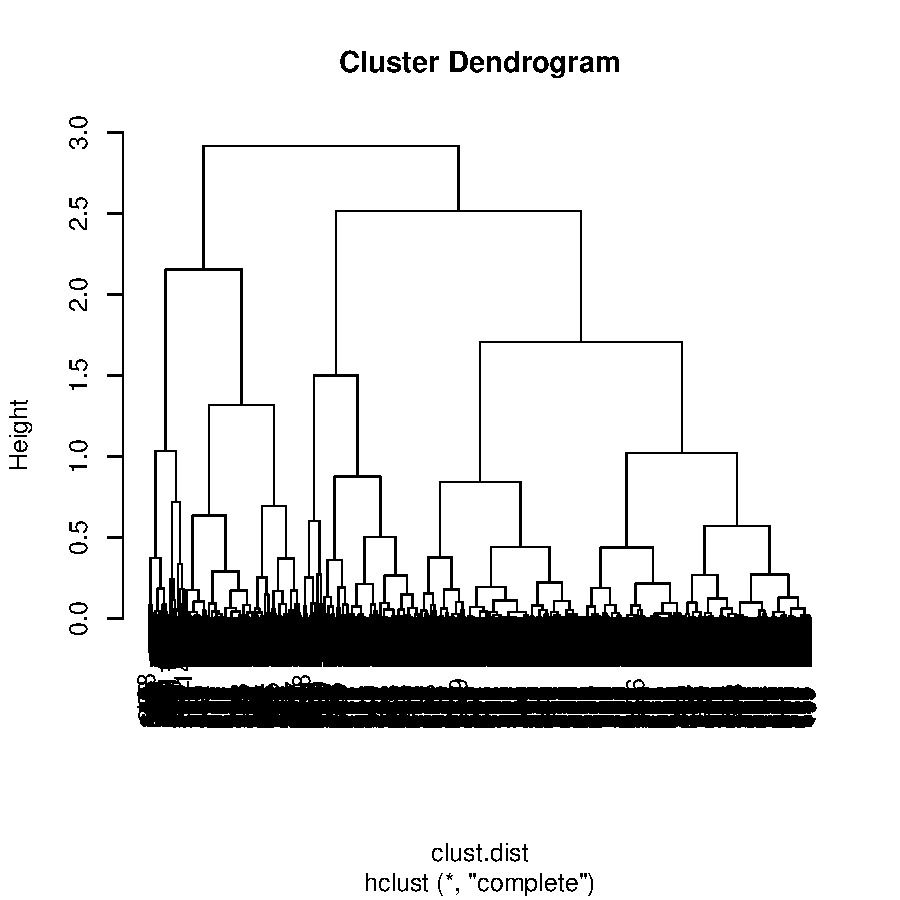
\includegraphics{project_report-011}

Next, we will look at a pairs plot that shows the paired relationships between the variables \texttt{price}, \texttt{latitude}, and  \texttt{longitude}. The points are coloured based on the 5 clusters that they were fitted to with the hierarchical clustering run above. Notice that the pyramid shape reflects what was seen in earlier reports. The $V$ shape between latitude and longitude reflects the actual layout of the map of New York City. Later on, we will see this mapped onto the geographic map to visualize it further. Overall here, the pairs plot shows that the clusters represent a stacked pyramid shape between \texttt{price} and \texttt{latitude} or \texttt{longitude}. It starts wide and short at the bottom, with many listings in the cheaper price range, and it narrows as it gets towards the top, which represents fewer listings in the higher price range.

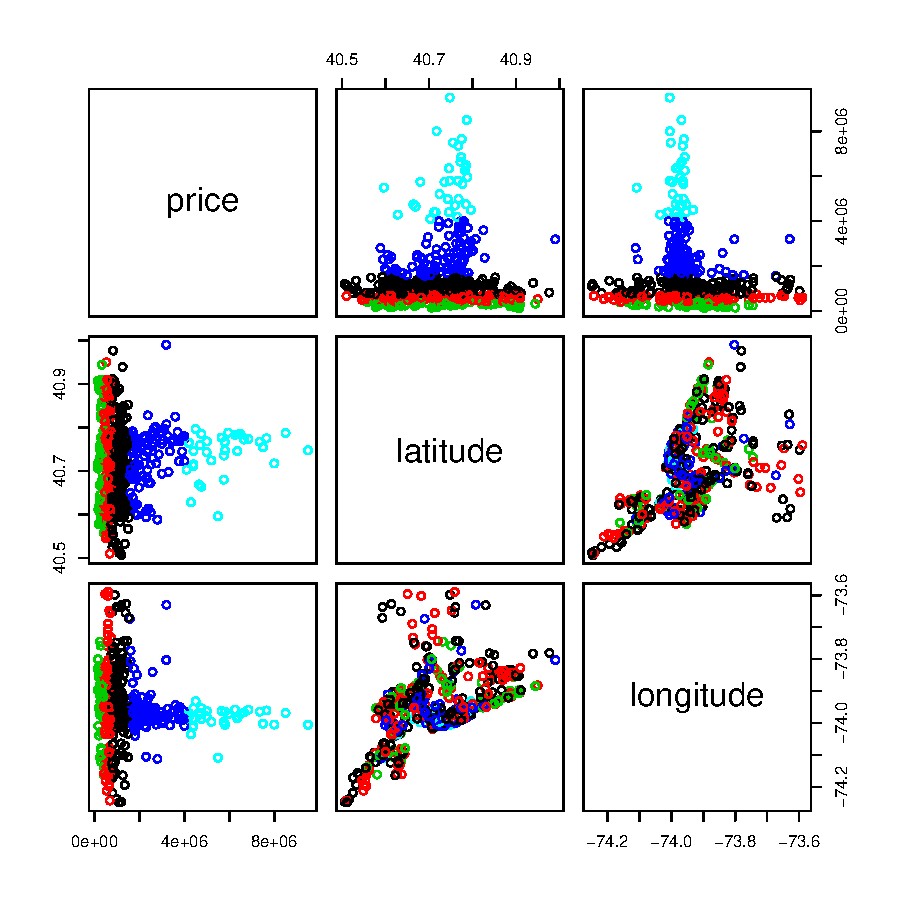
\includegraphics{project_report-012}

This next plot shows \texttt{longitude} and \texttt{latitude} on the x and y axis, respectively. Recall the $V$ shape here, which outlines roughly the layout of the city of New York, wrapping around the waterfront. The colours represent the hierarchical clustering assignments. Here it does not appear that the cluster assignments can be grouped by location (\texttt{latitude} and \texttt{longitude}) because they are scattered quite randomly throughout this plot.

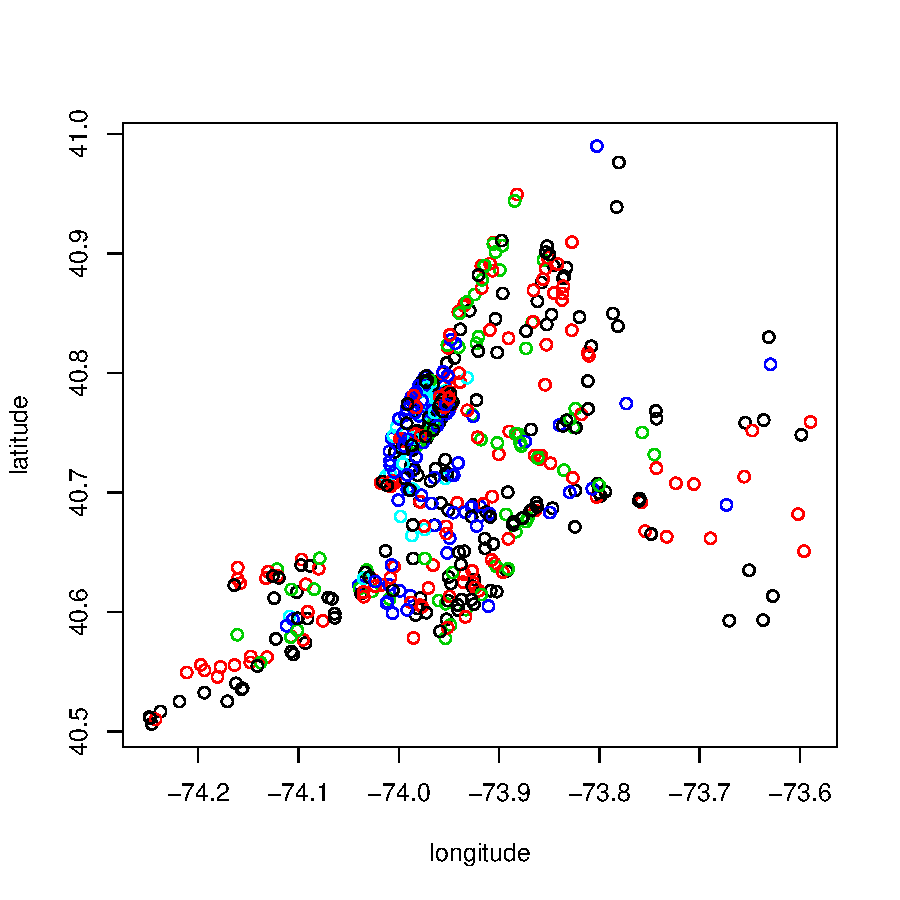
\includegraphics{project_report-013}



\pagebreak
\subsubsection{\textit{k}-means}

Next, \texttt{k}-means clustering was done. Note that \texttt{k}-means can only be conducted on data without missing values, so several rows were required to be removed in order to fit the data. Below, we see the pairs plot that shows the paired relationships between the variables \texttt{price}, \texttt{latitude}, and \texttt{longitude}. The points are coloured based on the new clusters fitted with the \texttt{k}-means clustering. Note the similar shape and colourings with the clusters appearing to form a pyramid shape between \texttt{price} and \texttt{latitude} or \texttt{longitude}. It starts wide and short at the bottom, with many listings in the cheaper price range, and it narrows as it gets towards the top, which represents fewer listings in the higher price range. Here, there appears to be a larger group at the bottom, in green. This green group looks thicker than the bottom green group in the hierarchical clustering. This indicates that \texttt{k}-means is fitting more values in that group than the hierarchical clustering did. The colouring of the clusters again seem to fit appropriately, similar to the hierarchical clustering above. The \texttt{latitude} and \texttt{longitude} also has the $V$ shape, following the layout of the city. We will look at this relationship further next.


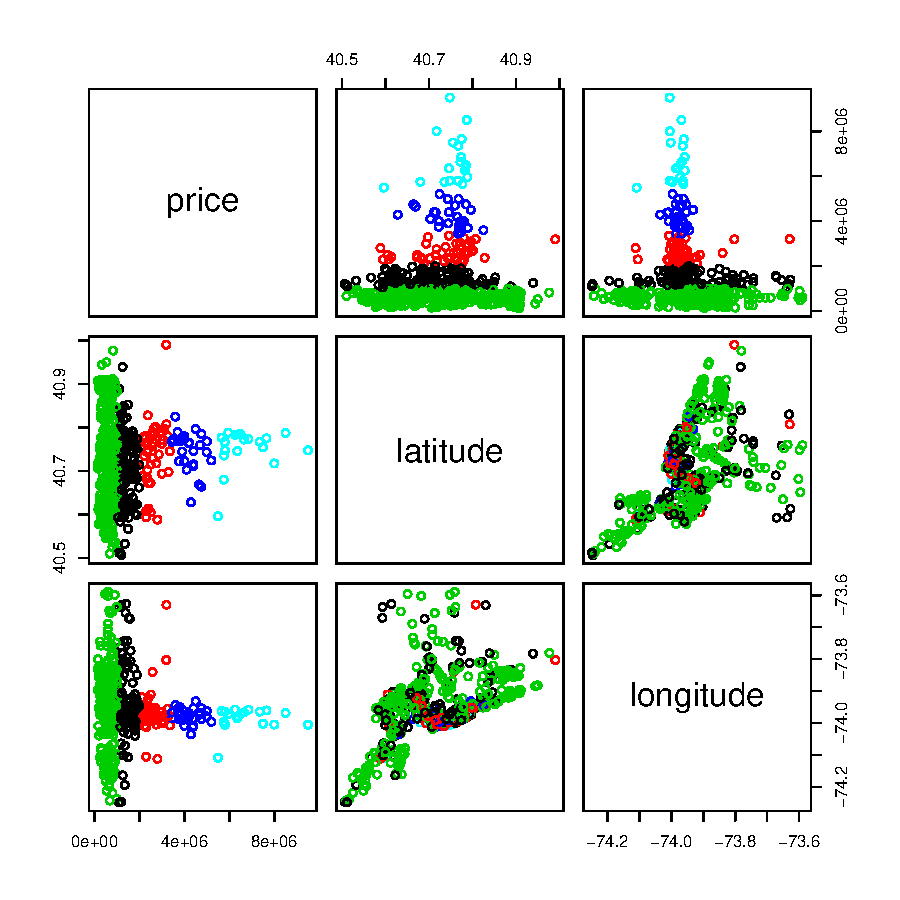
\includegraphics{project_report-015}

As mentioned, we will now look at a plot that shows \texttt{longitude} and \texttt{latitude} on the x and y axis, respectively. Again, like the hierarchical clustering, it does not appear that the cluster assignments can be grouped by location (\texttt{latitude} and \texttt{longitude}) because they are scattered quite randomly throughout this plot. The green appears to be the dominant cluster with the most points, and note that in the pairs plot above it was the bottom tier for price, indicating that this is the cheapest cluster of listings, which makes sense why there are more of them. It indicates that listings in this price range can be found all across the city. 

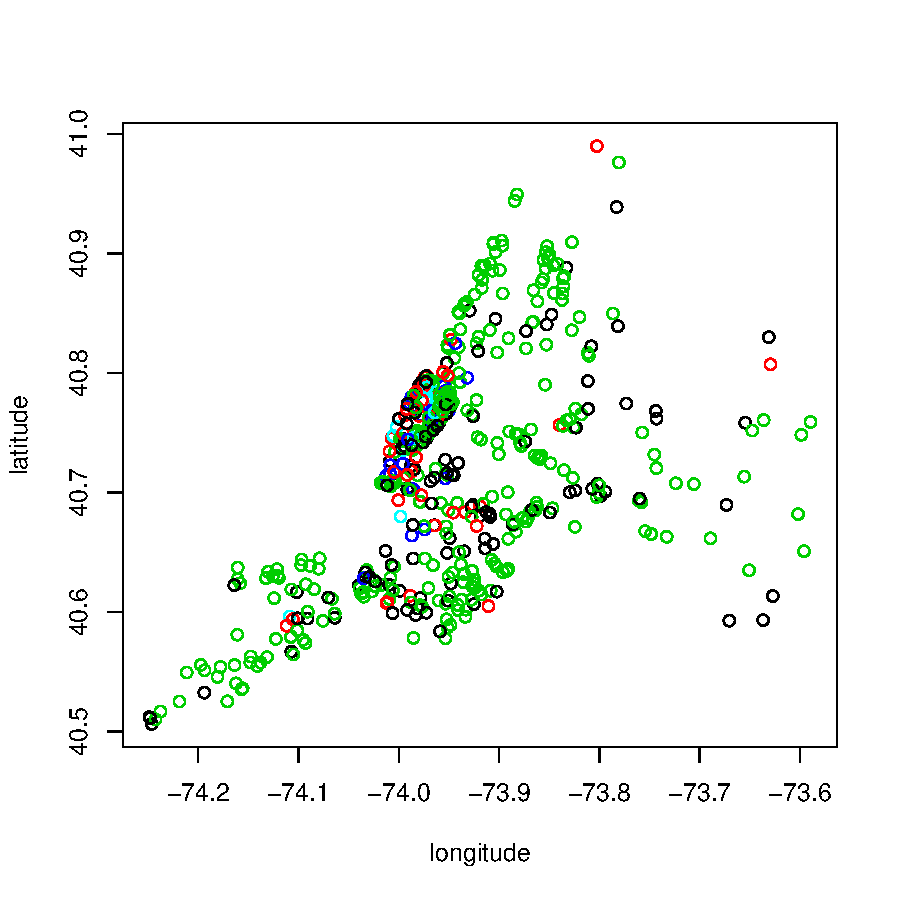
\includegraphics{project_report-016}

Next, the within sum of squares (WSS) was calculated for different values of $k$. This was plotted for all values $k$ from 1 to 15. See below for this plot. Notice that the WSS drops significantly from 1 to 2, and then plateaus around 4 or 5. This indicates that the ideal number of clusters to select from \texttt{k}-means clustering could be argued to be 5.

\begin{Schunk}
\begin{Soutput}
Plotting WSS for different k:
\end{Soutput}
\end{Schunk}
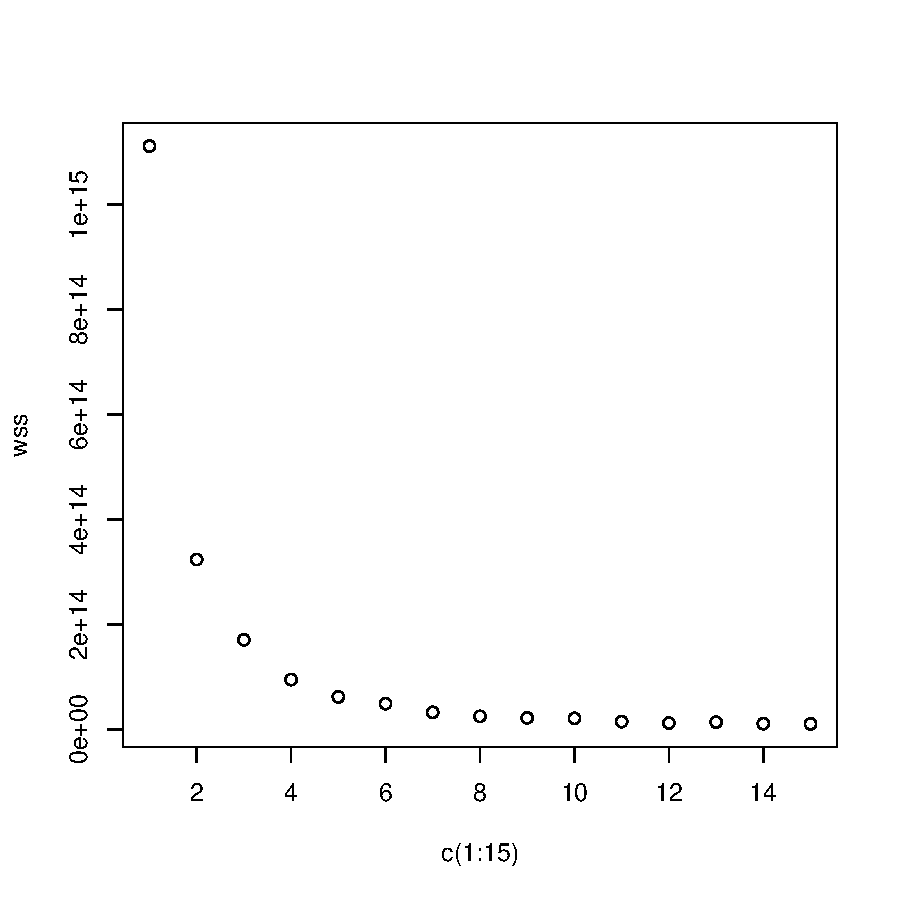
\includegraphics{project_report-017}


\pagebreak
\subsubsection{Mixture Models}

Next, mixture modelling was considered. Note that this can only be conducted on data without missing values, so several rows were required to be removed in order to fit the data. Below we see the plot that shows \texttt{longitude} and \texttt{latitude} on the $x$ and $y$ axis, respectively. The colouring of the points represent the groupings assigned by the mixture model. There were 5 groups selected to be fitted here. The value 5 was chosen to ideally model the 5 different boroughs in New York City. This plot appears to better outline different geographical locations compared to hierarchical clustering and \texttt{k}-means. However, there is still a lot of overlap between the clusters, and it does not have 5 distinct clusters that could outline the 5 boroughs. To improve this, we will play around with the number of groups fitted.

\begin{Schunk}
\begin{Soutput}
Mixture Model Clustering with 5 Groups:
\end{Soutput}
\end{Schunk}
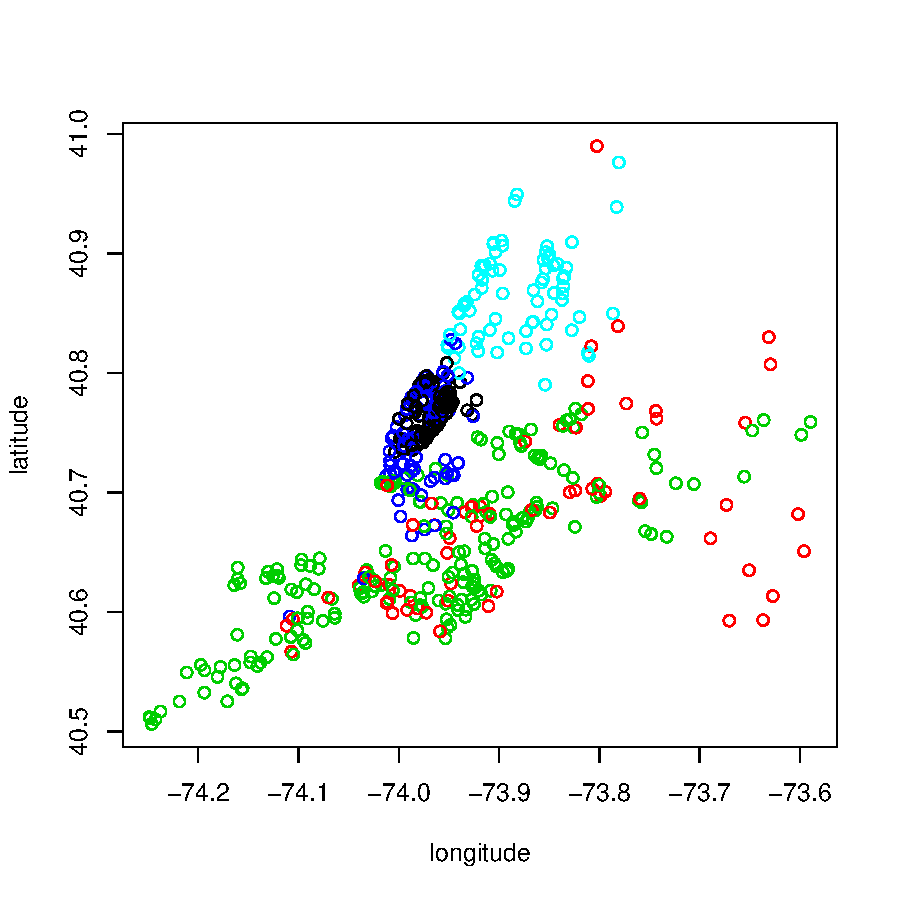
\includegraphics{project_report-018}



For some reason, the plot of \texttt{latitude} and \texttt{longitude} appears to better align with the 5 boroughs when there are 6 groups fitted to the mixture model. Below, we see the same plot but with the mixture model fitted to 6 groups. Here we see a distinct 5 groups in a shape and pattern that appears to follow the map of New York City. This is an interesting result, and could be occurring because the borders of the boroughs are closely aligned, and could cause confusion with the oddly shaped borders, as well as the fact that the water creates a sharp border on the other side. 

\begin{Schunk}
\begin{Soutput}
Mixture Model Clustering with 6 Groups:
\end{Soutput}
\end{Schunk}
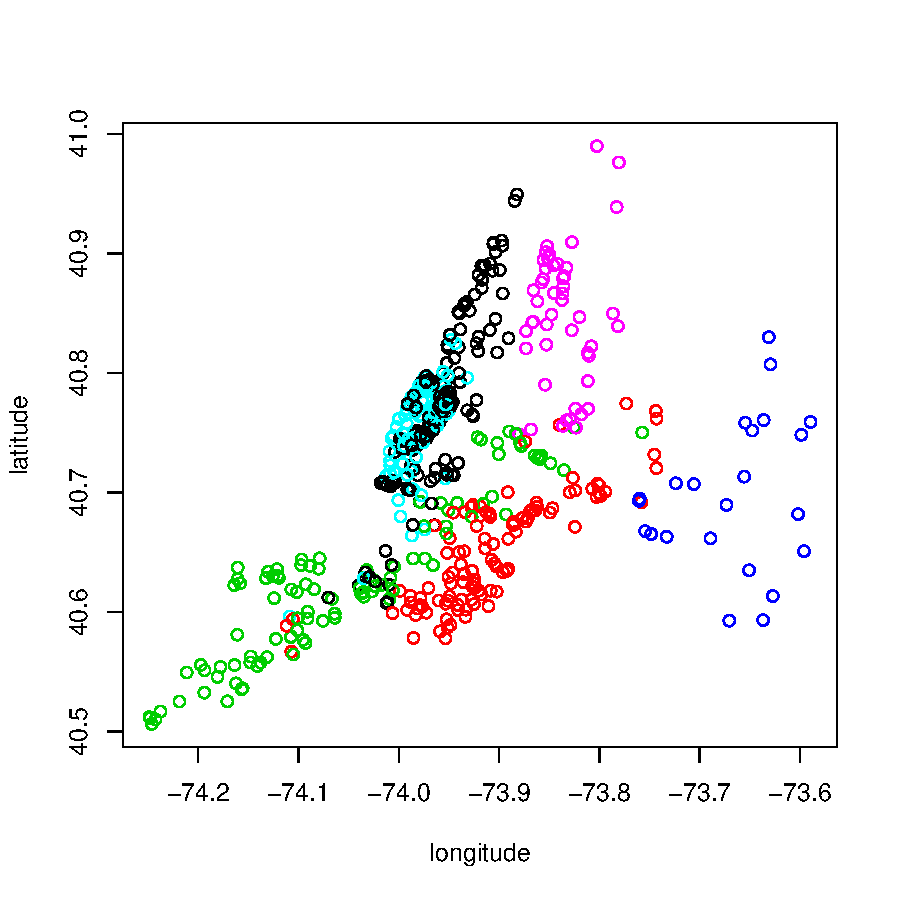
\includegraphics{project_report-019}



%Between 25-45, 25 was selected by Mclust:



To further visualize the above mixture model plot with 6 groups fitted, we can overlay this with the actual map of New York City, outlining the 5 boroughs. See below the map, with labels outlining the 5 different NYC boroughs. The points are coloured to reflect the cluster assignment. The labels are coloured to reflect the cluster-assigned groups. Notice that the points fit reasonably well within the map itself, and they roughly reflect the borough boundaries. Again, the $x$-axis represents \texttt{longitude} and the $y$-axis represents \texttt{latitude}.

\begin{Schunk}
\begin{Soutput}
Overlaying Borough Coordinate Boundaries:
\end{Soutput}
\end{Schunk}

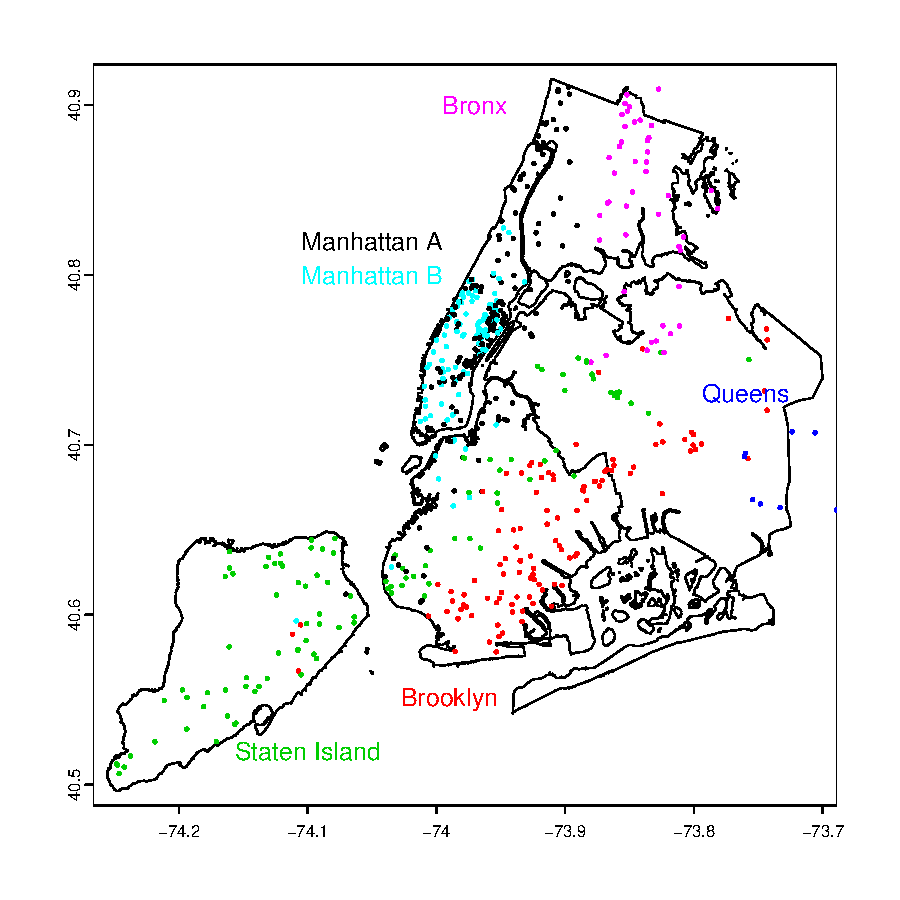
\includegraphics{project_report-022}



Recall that there are only 5 boroughs in New York City, but this model fitted 6 clusters. To understand the misclassification rate of the cluster assignments, we can view the classification table. The columns represent the actual borough that the listing belongs to, as calculated given the address of the listing. The rows represent the assigned borough from the mixture model classification assignments. Notice that the additional group, as there were 6 groups instead of the actual 5, splits into Manhattan A and Manhattan B. This was labelled as such because the points overlaped within the existing borough Manhattan. The misclassification rate is approximately 0.29. This is still relatively high for a misclassification rate, which is not ideal. See the table below for exact assignments and comparisons.

\begin{Schunk}
\begin{Soutput}
Classification Table:
\end{Soutput}
\begin{Soutput}
               true
mixclass        Bronx Brooklyn Manhattan Queens Staten Island <NA>
  Bronx            33        0         0     12             0    4
  Brooklyn          0       83         0     26             4    0
  Manhattan A      24       31       129      4             1    2
  Manhattan B       0        9        92      0             1    0
  Queens            0        0         0      5             0   18
  Staten Island     0       33         0     19            57    0
\end{Soutput}
\begin{Soutput}
Misclassification Rate: 0.2912966
\end{Soutput}
\end{Schunk}


\pagebreak

\section{Conclusions \& Recommendations}

Modelling price was relatively successful with the non-parametric approach. Recall our MSE was the lowest in this model, and the $R^2$ was significantly better here as well. We were correct in assuming that bed and bath would be important variables to determine price, but we incorrectly assumed that distance and feet would also be significant. The model represented the variation much better than we expected, given that we did not expect anything to perform well compared to the clustering approach.

Mapping pricing into clusters based on the distance variables also proved to be relatively successful. Although the misclassification rate was 0.29 for our best fitting cluster via mixture modelling, it still held up relatively well. Our hypothesis that this would be the best for mapping values onto the existing boroughs was also correct that the latitude and longitude would assist in this model. We hypothesized that price would be more significant to the specific boroughs, but it was not, as it was fairly evenly distributed based on regions, which was shown in our earlier clustering (hierarchical and k-means).

We came across a few issues in the beginning of the project with data collection, as well as outlier determination. This was outlined in the previous report. Specifically, the outlier distance calculation was very complicated due to missing values so it left us to calculate each variable individually rather than all variables in each row.

The model is currently restricted to the New York City data, so it could not be tested or used to make predictions on a different dataset. In the future, we would hope to train the model with different geographic locations to make it a more well-rounded model. Also, to improve the model we could add many more data points, as we were limited to approximately 800 here. Expanding the dataset would allow us to better train and test both the parametric and mixture model. Additionally, adding other features such as a binary variable if there is a view or not in the listing could also be beneficial. Distinguishing between condos and apartments and houses could also help improve the model, as it would consider that some apartments or condos could have strata fees which are not accounted for in the list price of a home, but are definitely considered by buyers when making purchase decisions.

Overall, the models explain the variance in the data relatively well. Although we have not tested the model to predict prices of a test set or on future data, that would be something to be explored in the future to further evaluate the success of the models fitted.

\end{document}
